% Files using this must be two subfolders
% deep. Adjust the number of ../ for the
% depth of the file.
% Imports
\usepackage{fancyhdr}
\usepackage{geometry}
\usepackage{icomma}
\usepackage{amsmath}
\usepackage{multicol}
\usepackage{mathptmx}
\usepackage{anyfontsize}
\usepackage{t1enc}
\usepackage{tabto}
\usepackage{listings}
\usepackage{filecontents}
\usepackage{subcaption}
\usepackage{tikz}
\usepackage[parfill]{parskip}
\usepackage{graphicx}
\usepackage[]{mdframed}
\usepackage{amsmath}
\usepackage[makeroom]{cancel}
\usepackage{pgfplots}
\usepackage{pgfplotstable}
\usepackage{xfrac}
\usepackage{amssymb}
\usepackage{mathtools}
\pgfplotsset{compat=1.18}
\usetikzlibrary{patterns}
\usepgfplotslibrary{polar}
\usepgfplotslibrary{fillbetween}

\geometry{margin=2.5cm}

\newcommand{\name}{Kaleb Burris}
\newcommand{\classname}{MATH F253, Elizabeth S. Allman, University of Alaska Fairbanks}
\newcommand{\assignment}{FILL IN ASSIGNMENT NAME}

\pagestyle{fancy}

\fancyhead[L]{
    \name 
    \newline
    \classname
    \newline
    \assignment
}

\newcommand{\horizontal}{\noindent\rule{\hsize}{0.4pt}}

\setlength{\headheight}{42pt}
\setlength{\headsep}{0.25in}
\setlength{\columnsep}{0.35cm}
\setlength{\columnseprule}{1pt}

\usepackage[T1]{fontenc}
\usepackage{lmodern}


\graphicspath{ {./lab08images/} }

% Put class number, class name, and professor 
% name.
% Use only in case of emergency, this
% should be covered by the preamble.
% \renewcommand\classname{}

% Put the assignment name with \S if 
% necessary for the section and the question 
% numbers.
\renewcommand\assignment{Lab 8: Torque, Angular Acceleration, and Moment of Inertia, 3/28/2023, Partners: Maite Valentin-Lugo, Seth Waln}

\begin{document}

    % Templates
    \iffalse
    % Use these for equations.
    \begin{equation*}
        \begin{gathered}
            Equations go here.
        \end{gathered}
    \end{equation*}

    % Use this if a line of math is too long.
    \resizebox{\hsize}{!}{$Long equation goes here$}

    % Use these for multiple columns.
    \begin{multicol*}{# of columns}
        % Remove the * if you want the columns to be balanced.
    \end{multicol*}

    % Use this to add a horizontal line.
    \horizontal

    \fi

    % Begin homework here.
    %%%%%%%%%%%%%%%%%%%%%%

    \begin{itemize}
        \item [1., 2.]~\\
        
        \begin{center}
            \begin{tabular}{l | l | l | l}
                   & Distance & Force & Torque  \\ \hline
                d1 & 0.398 & 0.493 & 0.196214   \\ \hline
                d2 & 0.375 & 0.507 & 0.190125   \\ \hline
                d3 & 0.348 & 0.541 & 0.188268   \\ \hline
                d4 & 0.324 & 0.555 & 0.17982    \\ \hline
                d5 & 0.298 & 0.587 & 0.174926   \\ \hline
                d6 & 0.274 & 0.622 & 0.170428   
            \end{tabular}
        \end{center}

        \item[3.]~\\
        
        {\centering\resizebox{0.9\hsize}{!}{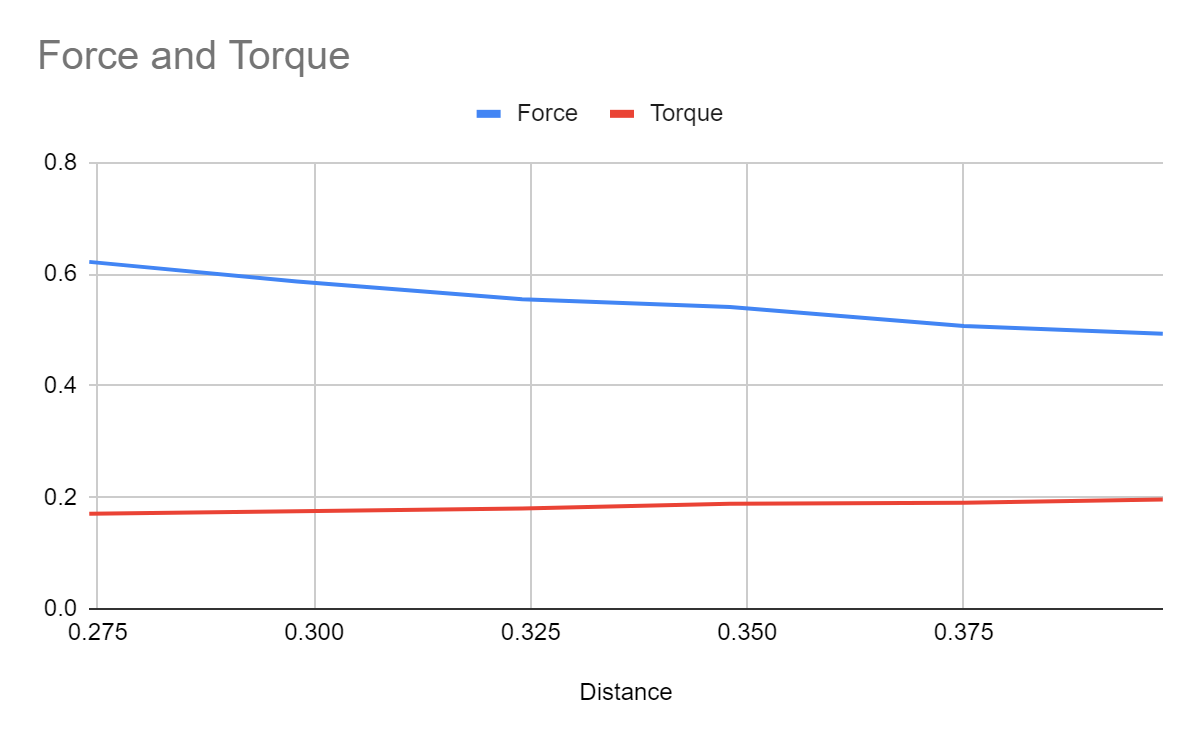
\includegraphics{image18}}}

        \item[4.]~\\
        
        \begin{center}
            \begin{tabular}{l | l | l | l}
                & Disk & ball & Ring                    \\ \hline
                Diameter (m)& 0.0960 & 0.0987 & 0.0990  \\ \hline
                Mass (kg)   & 0.5275 & 0.7462 & 0.2109
            \end{tabular}
        \end{center}

        \item[5.]~\\
        
        \begin{center}
            \begin{tabular}{l | l}
                & Inertia                   \\ \hline
                Ring        & 0.0005167  \\ \hline
                Ball        & 0.0007292  \\ \hline
                Disc        & 0.0006076
            \end{tabular}
        \end{center}

        \item[6.]
        
        Ring - Seth

        Ball - Maite, Kaleb

        \item[7.]
        
        The ball won the race.

        \item[8.]
        
        Yes, I believe the low surface contact between the ball and the ramp led to lower energy loss to friction, it also had a higher mass but a similar radius to the others, meaning its initial potential energy was higher, and it had the highest theoretical inertia.

        \item[9.]
        
        \begin{center}
            \begin{tabular}{|l|l|l|l|}
            \hline
                 & Ring & Disk & Sphere \\ \hline
                Initial position (when velocity is zero) & 0 & 0 & 0 \\ \hline
                Position at measurement of final velocity & 2 & 2 & 2 \\ \hline
                Height difference at measurement of final velocity & 0.125 & 0.125 & 0.125 \\ \hline
                Final Velocity & 1.172 & 1.181 & 1.366 \\ \hline
                Final Angular velocity & 0.0422 & 0.0406 & 0.0361 \\ \hline
            \end{tabular}
        \end{center}

        \item[12.]
        
        \begin{align*}
            K_{i} + U_{i}               
            & = K_{f} + U_{f}                           \\
            \frac{1}{2}I\omega^{2}_{i} + mgh_{i} 
            & = \frac{1}{2}I\omega^{2}_{f} + mgh_{f}    \\
            \frac{1}{2}I(0) + mgh_{i}
            & = \frac{1}{2}I\omega^{2}_{f} + mgh_{f}    \\
            -\frac{1}{2}I\omega^{2}_{f}
            & = mgh_{f} - mgh_{i}                       \\
            I
            & = \frac{2mg(\Delta h)}{\omega^{2}_{f}}
        \end{align*}

        \item[13.]~\\
              
        \begin{center}
            Computed in excel $\implies$ 
            \begin{tabular}{l | l}
                & Inertia             \\ \hline
                Ring        & 289.65  \\ \hline
                Ball        & 782.35  \\ \hline
                Disc        & 1400.71
            \end{tabular}
        \end{center}

        \item[14.]
        
        Terribly. The calculated moments of inertia were about 7 orders of magnitude smaller, for the case of the ball, it was $\frac{1400.71}{0.00073} = 1,918,781$ times larger in the experimental case. I have no idea what we did in our calculations for this to happen, but it is astronomically wrong.

        \item[15.]
        
        I'm almost certain our equations were not set up correctly. On top of that, the obvious things like friction, vibration, and inaccuracy in where we dropped the objects, are all also factors in the uncertainty.

        \item [16.]
        
        Center - Kaleb

        \item [18.]
        
        If the wheels are lighter, it'll take less energy to move them, meaning you have to spend less energy accelerating/decelerating.

        \item [19.]
        
        The slower the discus spins, the less rotational acceleration will occur, which will pull the discus back and forth, reducing its overall horizontal speed.

        \item [20.]
        
        I don't know what a moment of inertia stick is, we didn't engage with them.

    \end{itemize}

\end{document}